
\section{CHAPTER 1 : FAT32}
\subsection{Đọc Boot Sector}

Tạo một Class \textbf{BootSector} thuộc file BootSector.h dùng để đọc các sector trong phân vùng thành một ma trận có kích thức 32x16 \\
\indent
Sử dụng con trỏ bootSector trỏ tới hàm \textbf{getBootSector} của file \textbf{system.h} dùng để đọc sector đầu tiên của phân vùng và trả về một bảng bootSector 512byte kích thước 32*16\\
\indent
Khai báo một class \textbf{IValueMapper} dùng để tạo một lưu trữ các thông tin bằng thư viện map. Để lấy được các thông tin cần thiết từ bảng bootSector ta khởi tạo một con trỏ kiểu \textbf{IValueMapper( IValueMapper* mapper = new BootSectorMapper)} dùng con trỏ này để trỏ đến các hàm chức năng thuộc class \textbf{bootSectorMapper} trong file \textbf{BootSectorMapper.h}.\\
\indent 
Sau đó, khai báo  \textbf{map<string,int> bootSectorMapper} để lưu lại các thông tin khi sử dụng con trỏ Mapper trỏ đến hàm mapper truyền vào hàm một bảng bootSector kiểu \textbf{string**(map<string, int> bootSectorMapper = mapper->mapper(bootSector) )} hàm mapper thuộc class BootSectorMapper có chức năng ánh xạ bảng bootSector vừa có ở trên ra các thông tin cần thiết như SC,SB,nF,SR,SV,SF,SB,... Để tìm được các thông tin từ bảng bootSector ta sử dụng thư viện chuẩn namespace \textbf{Utils} thuộc file header \textbf{Utils.h} chứa các class Int dùng để chuyển đổi từ kiểu Hex sang kiểu Decimal.\\

\begin{figure}[htp]
    \centering
    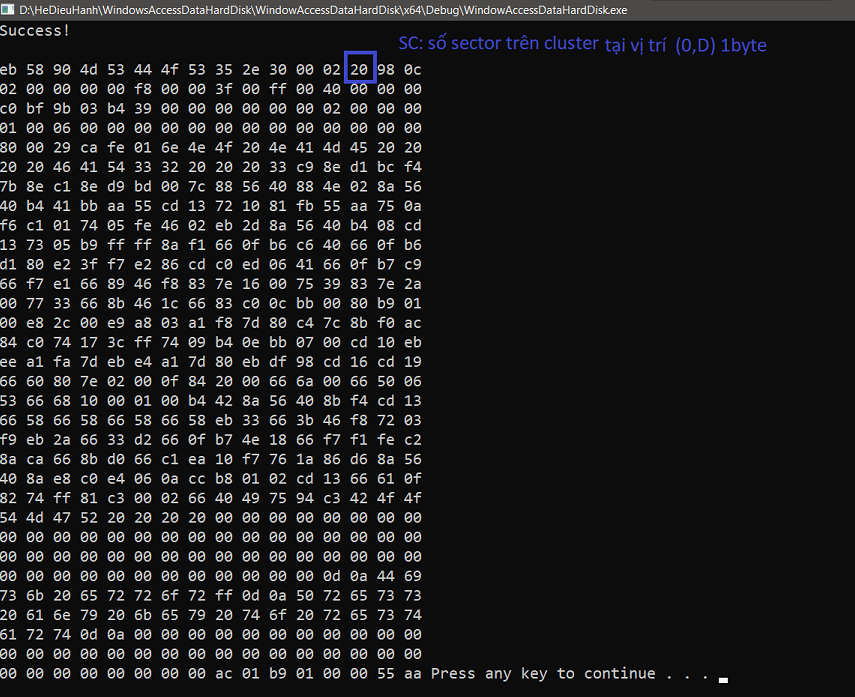
\includegraphics[scale=.5]{CHAPTER 1/Images/SC.png}
    \caption{Số Sector trên Cluster}
    \label{fig:my_label}
\end{figure}

\subsection{Đọc bảng FAT}
\noindent
Các obj dùng trong sector này: FatTable, FatTableMapper, ReadFatTable\\
\indent
\textbf{FatTable} : cài đặt sector và các bảng fat tương ứng\\
\indent
Tạo class FatTable gồm các atribute :\\
\indent\indent
+ \textbf{\_numberofSector} : cho biết số Sector có trong hàm \\
\indent\indent
+ \textbf{fatTable} : mô tả bảng fat của các sector tương ứng\\
\indent
\textbf{FatTableMapper::mapper(Object* origin)}(\#\#) (được kế thừa từ class IValueMapper): dùng để truy xuất các phần tử theo fat32 bằng cách dùng map để ánh xạ. Cụ thể như sau:\\
\indent
Được truyền vào 1 obj là 1 FatTable sau đó ánh xạ từ vị trí đến giá trị của bảng fat tại vị trí đó. \\
\indent
Tức là với i miễn là bé hơn SECTOR\_ROW ( trong trường hợp này là 16) thì máy tính sẽ tiếp tục thao tác. Máy tính sẽ lấy 4 byte(do trong fat32 mỗi phần tử có 4 byte) kế tiếp nhau theo thứ tự ngược lại ( từ 3 về 0, đó là lí do tại sao biến col có giá trị 3). \\
Sau khi có chuỗi 4 byte này ( lúc này đang ở dạng hexa ), chúng sẽ được dịch sang decimal ( đây chính là giá trị của 1 phần tử FAT). 
ctdl mp sẽ ánh xạ biến index là stt phần tử FAT tới giá trị của nó sau đó tiếp tục cộng lên và chuỗi buffer.str được reset lại.\\
{\textbf ReadFatTable::Read(int point)}\\
trước khi đi sâu vào phân tích hàm này chúng ta hãy tìm hiểu những thông tin khác!
\textbf {File System.h}\\
\textbf {getBootSector()} hàm này dùng để "đọc" và trả về 1 Sector chứa toàn bộ thông tin vừa đọc được\\
\textbf {ReadSector()} hàm này dùng cho công việc "đọc" đã nói ở trên, cụ thể như sau:\\
\indent
Sau khi kiểm soát lỗi không mở được device hoặc không đặt được file và đặt điểm bắt đầu để đọc, hàm bắt đầu quy trình đọc.\\
\indent
Hàm cấp phát động 1 mảng sectors 2 chiều sau đó duyệt từng phần tử của mảng 512 phần tử (ở đây ta hiểu là bảng fat32 gồm 512 byte được truyền vào ) sau đó trả về 1 sector chứa đầy đủ thông tin đã được đọc.\\
Quay trở lại hàm Read(int point)\\
\textbf{ mapper} dùng để ánh xạ ta đã nói ở trên (\#\#)\\
nếu bảng fat không tồn tại để đọc, hàm sẽ tạo ra 1 sector chứa 1 bảng fat\\
nếu bảng lớn hơn 1 sector, deepcopy sang 1 newFatSector với kích thước mới, sau đó swap 2 bảng với nhau rồi xóa bảng cũ, lúc này bảng fat mà chúng ta đang sử dụng không khác gì lúc đầu, chỉ có kích thước to hơn. Sau đó tiếp tục insert thêm dữ liệu mới vào.\\
sau mỗi thao tác như vậy hàm liên tục kiểm tra xem đã đến cuối cùng của bảng fat chưa, nếu rồi thì break vòng lặp, trả về fatTable và kết thúc hàm.\\
\subsection{Đọc bảng RDET}
\noindent
các obj dùng trong sector này: ReadDirectoryTable, RootDirectoryTable, 
 map<string, int> bootSectorMapper = mapper->mapper(bootSector);\\
\textbf{ int point = bootSectorMapper["Sb"] + bootSectorMapper["Nf"] * bootSectorMapper["Sf"];}\\
\indent
Khi đã lưu được thông tin cần thiết từ bảng bootSector vào trong bootSectorMapper thì ta sẽ tính địa chỉ sector đầu tiên có trên RDet bằng công thức Sb+Nf*Sf và lưu nó vào một biến point kiểu int.\\
\indent
Khai báo con trỏ reader kiểu ReadDirectoryTable(ReadDirectoryTable* reader = new ReadDirectoryTable()) thuộc class ReadDirectoryTable trong file ReadDirectoryTable.h dùng để đọc các thông tin của bảng thư mục gốc. 	\\
\indent
Khai báo con trỏ directory kiểu DirectoryTable thuộc class DirectoryTable trong file DirectoryTable.h dùng để lưu trữ các thông tin đã đọc được từ hàm Read(Point) của class ReadDirectoryTable.\\
\indent
khai báo con trỏ RDET kiểu RootDirectoryTable thuộc class \textbf{RootDirectoryTable} trong file \textbf{RootDirectoryTable.h} dùng để lưu trữ thông tin các entry con khi truy xuất từ bảng thư mục gốc và lưu vào một vector<Entry*> \_entrys để dễ dàng sử dụng các thông tin từ các entry này\\
\subsubsection{Đọc entry chính}
\noindent
các obj trong sector này: MainEntry, \\
\indent
Để đọc được entry chính của bảng thư mục gốc ta tiến hành bằng cách truyền vào trong hàm \textbf{Read} thuộc class \textbf{ReadDirectoryTable} một biến Point kiểu int(Địa chỉ sector đầu tiên RDET) trong hàm chức năng này ta khởi rạo một mảng string hai chiều có tên directory dùng để lưu thông tin của bảng thư mục gốc, sau đó kiểm tra xem bảng thư mục gốc có một hay nhiều hơn một sector nếu nhiều hơn một sector thì khởi tạo một mảng string hai chiều có tên newDirectory để lưu trữ tạm thời thông tin của sector và sau đó mới chèn các giá trị của sector vào mảng directory. \\
\indent
Để kiểm tra xem khi nào bảng thư mục gốc kiểu thúc ta sử dụng một hàm bool \textbf{ReadDirectoryTable::\\isEndOfDirectory(string** sector)} nếu giá trị của sector tại thời điểm đó truyền vào bằng 0 thì sẽ ngừng truy xuất bảng thư mục gốc.
khi đã có được thông tin của các sector thuộc bảng thư mục gốc ta tiến hành kiểm tra xem sector nào là thư mục chính bằng khởi tạo một mảng string hai chiều có tên entryTable dùng để lưu thông tin của từng sector có kích thức 2x16 kiểm tra xem tại vị trí (0,11) nếu là '02' thì đó là thư mục chính và sau đó phân tích các thông tin cần thiết của entry chính(chèn hình kèm hướng dẫn)  khai báo class \textbf{MainEntry} thuộc file \textbf{MainEntry.h} để hiển thị các thông tin của entry chính ra màn hình.\\
\subsubsection{Đọc entry phụ}
các obj trong sector này: SubEntry\\
Cũng giống như entry chính nhưng để kiểm tra xem entryTable có là một thư mục tên dài hay không thì tại vị trí (0,11) nếu là '0F' thì đó là entry phụ  sau đó phân tích các thông tin cần thiết của entry phụ(chèn hình kèm hướng dẫn)  khai báo class\textbf{ SubEntry} thuộc file \textbf{SubEntry.h} để hiển thị các thông tin của entry phụ ra màn hình.
\subsubsection{Tạo folder, file}
tạo folder và file bằng hàm init của obj Cfolder:\\
Kiểm tra vector \_item có trùng lặp hay không bằng cách kiểm tra \_item có trống hay không, nếu không trống thì return. Lấy sector chứa thông tin bằng hàm \textbf{getBootSector} và lưu vào trong \textbf{bootSectorMapper}. Sau đó tính địa chỉ sector đầu tiên có trên RDet bằng công thức \textbf{Sb+Nf*Sf} và lưu nó vào một biến indexSector kiểu int. \\
Khai báo con trỏ reader kiểu ReadDirectoryTable(ReadDirectoryTable* reader = new ReadDirectoryTable()) thuộc class \textbf{ReadDirectoryTable} trong file \textbf{ReadDirectoryTable.h} dùng để đọc các thông tin của bảng thư mục gốc. 	
Khai báo con trỏ directory kiểu DirectoryTable thuộc class \textbf{DirectoryTable} trong file \textbf{DirectoryTable.h} dùng để lưu trữ các thông tin đã đọc được từ hàm \textbf{Read(intdexSector)} của class \textbf{ReadDirectoryTable}.\\
 Đọc và lưu các entry vào \textbf{vector<Entry*>vtEntry} bằng con trỏ RDET kiểu RootDirectoryTable để thao tác. Sau đó duyệt từng block entry để lấy thông tin và kiểm tra entry đó là file hay folder, để tạo file hoặc folder tương ứng với thông tin từ vtEntry và thêm vào vector \_item. 
\subsection{Render màn hình}
Gồm các hàm chính :ConsoleColor, ConsoleModifySetColor, ...\\
ConsoleColor là class đảm nhiệm vị trí render màn hình.\\
Hàm ConsoleColor chỉ định màu nền cho Console ( ở đây màu mặc định là 7 - màu trắng, nhưng chúng ta có thể điều chỉnh thành các màu khác theo sở thích)\\
bên cạnh đó việc truyền vào nhiều biến hơn cũng có thể điều chỉnh chữ và cả màu nền
với công thức \textbf{this->\_consoleColor = textColor + backgroundColor * 16}, ta có thể tùy chỉnh tùy thích theo bảng sau :\\
\indent\indent\indent
    0 = Black   \quad    8 = Gray\\\indent\indent\indent
    1 = Blue   \quad     9 = Light Blue\\\indent\indent\indent
    2 = Green    \quad   A = Light Green\\\indent\indent\indent
    3 = Aqua     \quad   B = Light Aqua\\\indent\indent\indent
    4 = Red       \quad  C = Light Red\\\indent\indent\indent
    5 = Purple    \quad  D = Light Purple\\\indent\indent\indent
    6 = Yellow    \quad  E = Light Yellow\\\indent\indent\indent
    7 = White    \quad   F = Bright White\\
\subsection{vẽ cây thư mục}
hàm progarm trong file cpp dùng để thao tác với cây thư mục. Khi chương trình chạy sẽ hiện ra thông tin của thư mục fat32 và bao gồm các file và folder. Sử dụng các phím mũi tên và enter để chọn file hoặc folder, khi chọn file thì sẽ có tên, thông tin và nội dung, nếu nội dung trống thì sẽ xuất "SYSTEM: FILE EMPTY"; khi chọn folder thì sẽ hiện tên, thông tin và các file mà folder đó chứa. Sử dụng phím esc để thoát.